\section{Künstliche Intelligenz}

\gls{ki} gewann in den letzten Jahrzehnten immer mehr an Beliebtheit und ist im Alltag stets vertreten (auch in Situationen, wo man sie nicht erwartet), jedoch ist diese Art von Technologie keine Neuheit. Erstmals wurde der Begriff \Gls{ki} von McCarthy im Jahr 1956 erwähnt, welcher auf der Dartmouth Universität ein Forschungsprojekt zu diesem Thema führte. \cite{100YAI} Dazu kommen noch Begrifflichkeiten wie \gls{ml} und \gls{dl}, welche oftmals als Synonym verwendet werden, allerdings handelt es sich dabei um eigene Bereiche, die sich dennoch in vielen Aspekten überschneiden.

\begin{figure}[H]
    \centering
    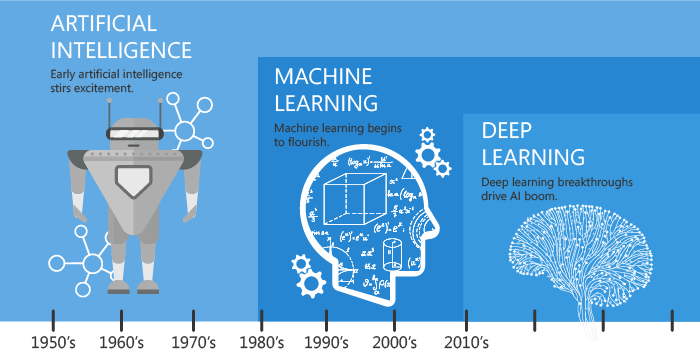
\includegraphics[scale=0.55]{sections/machine-learning/images/ki-ml-dl.png}
    \caption{Evolution von Künstlicher Intelligenz}
\end{figure}
%https://miro.medium.com/max/700/0*jng0i9svVVe7L7sj

Der Begriff \gls{ki} (\gls{ai}) lässt sich nur schwer genau definieren und umfasst daher ein breites Spektrum der Informatik. Dabei wurden im Verlauf der Geschichte mehrere Definitionen aufgestellt, welche sich auf die unterschiedlichen Interpretationen des Wortes ''Intelligenz'' fokussieren.

\begin{quote}
    Artificial intelligence is that activity devoted to making machines intelligent,
    and intelligence is that quality that enables an entity to function appropriately
    and with foresight in its environment. \cite{TQFAI}
\end{quote}

Diese Definition umfasst sowohl komplexe, als auch einfach verknüpfte Logiken wie ein Taschenrechner oder vorbestimmte Zuordnungen (Listing \ref*{lst:Zuordnung}). Jedoch repräsentieren diese Beispiele nicht den heutigen Fortschritt in diesem Bereich der Technologie.

\begin{lstlisting}[language=Java,caption={Zuordnung mit einer if/else-Verzeigung},label={lst:Zuordnung}]
    if(/* Bedingung */){
        // Funktionalitaet
    } else {
        // Funktionalitaet
    }
\end{lstlisting}

Da das Konzept der \gls{ki} nicht vorgibt, mit welcher Technik ein Problem gelöst wird, bestand die Möglichkeit einer Ausbreitung in allen möglichen Richtungen, welche sowohl Algorithmen als auch Einsatzgebiete inkludieren. Dabei gilt eine Voraussetzung: das Imitieren einer menschlichen Funktion.